\renewcommand{\thesection}{\Alph{section}}
\setcounter{section}{0}
\section{Appendix} \label{section:appendix}

\subsection{The Univariate Normal Distribution} \label{section:uninormal}
Let $x \sim \mathcal{N} \left( \mu, \sigma^2 \right)$. Then
\begin{eqnarray}
f(x) &=& \frac{1}{\sigma} \frac{1}{2\pi} \exp \left( \frac{-1}{2} \left( \frac{x - \mu}{\sigma} \right)^2 \right) \nonumber \\
     &=& \frac{1}{\sigma} \phi \left( \frac{x - \mu}{\sigma} \right) 
\end{eqnarray}
\noindent where $\phi(\cdot)$ is the p.d.f. of a univariate normal standard distribution.

\subsection{The Conditional Normal Theorem} \label{section:conditional}
Consider two random vectors, $\bf{x_{1}}, \bf{x_{2}}$, which are jointly, normally distributed:
\begin{equation}
\left[ \begin{array}{c}
\bf{x_{1}} \\
\bf{x_{2}} 
\end{array} \right]
\thicksim \mathcal{N}
\left[ \left( \begin{array}{c}
\bf{\mu_{1}} \\
\bf{\mu_{2}} 
\end{array} \right)
,
\left( \begin{array}{cc}
\bf{\Sigma_{11}} & \bf{\Sigma_{12}}  \\
\bf{\Sigma_{21}} & \bf{\Sigma_{22}}
\end{array} \right) \right]. 
\end{equation}
\noindent Then
\begin{equation}
\bf{x_{1}} | \bf{x_{2}} \thicksim \mathcal{N} (\bf{\mu_{1.2}},\bf{\Sigma_{11.2}})
\end{equation}
where
\begin{eqnarray}
\bf{\mu_{1.2}}     &=& \bf{\mu_{1}} + \bf{\Sigma_{12}}{\bf{\Sigma_{22}}}^{-1}(\bf{x_{2}}-\mu_{2}) \\
\bf{\Sigma_{11.2}} &=& \bf{\Sigma_{11}}   - \bf{\Sigma_{12}}{\bf{\Sigma_{22}}}^{-1}\bf{\Sigma_{21}}
\end{eqnarray}

\subsection{Constrained and Unconstrained Parameters} \label{conopt}
\noindent It is often the case that research questions involve constrained parameters. Constrained optimization methods, however, may not give satisfactory answers or may require to compute very complicated function gradients. There are ways to map constrained parameters into unconstrained parameters. This enables to use unconstrained optimization methods in constrained optimization problems, and avoids either insensible answers or infeasible computations. It prevents the optimization methods to go off. Think, for example, of a variance estimation. If the optimization algorithm searches in a region in which the variance is negative, the likelihood function, probably, takes a non-numeric value and the process stops without finding an optimum.\\
\indent For example, $\sigma_{\eta},\sigma_{\epsilon}$ are non-negative. Thus, it is necessary to find a method that maps a parameter $x \in (0,\infty)$ to a parameter $\tilde{x} \in (-\infty,\infty)$ and viceversa. In general, the following steps allow to deal with that:
\begin{enumerate}
\item Find a function $f(x)$ such that its range is identical to the domain of $x$ and its domain takes any value in the real line. 
\item Optimize based on $\tilde{x} = f(x)$. This is, set the initial condition based on $f^{-1}(x)$. 
\item Apply $f$ to $f^{-1}$ inside the definition of the objective function so that the calculations are based on the correct values, $x$.
\item Revert back the estimates through $f$.  
\end{enumerate}
\noindent Importantly, $f(\cdot)$ needs to be invertible for these steps to work.
\begin{example} (Non-Negativity Constraints) \label{ex:noneg}
It is necessary to estimate a parameter $x > 0$. The function $f(x) = \exp(x)$ has a range which is identical to the domain of $x$, its domain is the real line, and its inverse is the $\log(\cdot)$ function. Then, it is possible to use unconstrained optimization methods as follows:
\begin{enumerate}
\item If $\alpha$ is the initial condition the researcher has in mind, set $\log(\alpha)$ as the initial condition. This makes the optimizer understand that any value it tries for $x$ needs to be positive.
\item In order for the optimizer to evaluate the function in terms of $x$, redefine the objective parameter through the function $\exp(\cdot)$.
\item The optimizer finds $log(x^*)$. Apply $\exp(\cdot)$ to recover the parameter of interest.
\end{enumerate}
\end{example}

\begin{example} (Symmetric Interval Constraints)
In this case it is necessary to estimate a parameter, $x$, that lies in a symmetric interval, e.g. $x \in [-a,a]$ for  $a \in \mathbb{R}$. Note that the range of
\begin{equation}
f(x) = \left[ \frac{1}{1+ \exp(-x)} -.5 \right] \times 2 \times a
\end{equation}

\noindent is exactly $[-a,a]$, its domain is the real line, and its inverse is the following 
\begin{equation}
f^{-1}(x) = - \log \left[ \frac{2a}{x+a} - 1 \right].
\end{equation}
\noindent It is possible, then, to use the same algorithm as in Exercise \ref{ex:noneg}.
\end{example}

\begin{center}
\begin{figure}[H]
\caption{Symmetric Intervals Function for Different Values of $a$}
\centering
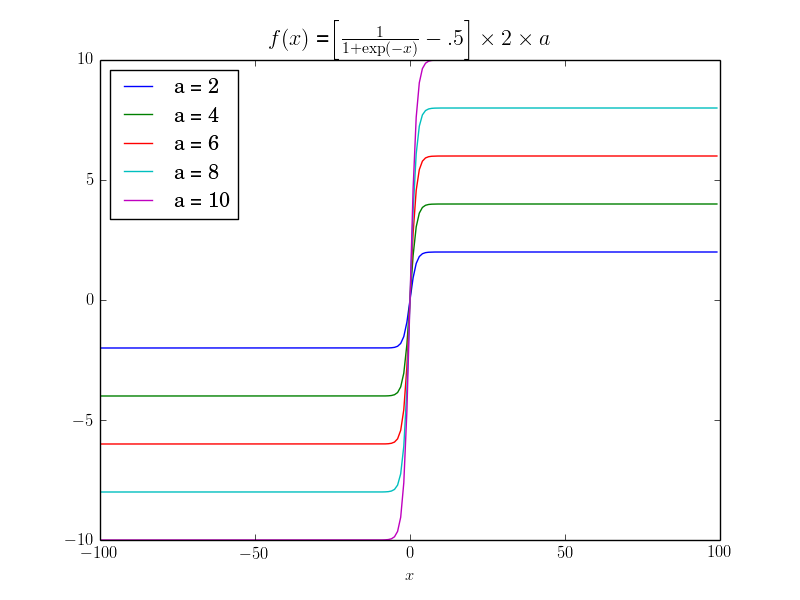
\includegraphics[width=4.5in, height=3.5in]{/home/jorge/Mine/econ350/StructuralEstimation/Handout/Solution/Code/other/symmetric_intervals.png}
\end{figure}
\end{center}

\indent This is relevant in the problem at hand. In particular, the estimands $\sigma_{\eta},\sigma_{\epsilon},\sigma_{\eta,\epsilon}$ need to satisfy
\begin{eqnarray}
\sigma_{\eta}^2 \times \sigma_{\epsilon}^2 &>& \sigma_{\eta,\epsilon}^2 \nonumber \\
&=& -\sigma_{\eta} \sigma_{\epsilon} < \sigma_{\eta,\epsilon} < \sigma_{\eta} \sigma_{\epsilon}
\end{eqnarray}

\noindent for the co-variance matrix of $\eta,\epsilon$ to be positive definite. If this restrictions are ignored and the initial conditions are arbitrary (i.e., the researcher ignores how the data generating process behaves and the initial conditions are a guess) the optimization routine may fail to have success. See the codes ``womansestimation.py'' and ``womandestimation.py'' to clarify how this works in practice.

